\documentclass[a4paper]{article}

\usepackage{inputenc}
\usepackage[british,UKenglish]{babel}
\usepackage{amsmath}
%\usepackage{titlesec}
\usepackage{color}
\usepackage{graphicx}
\usepackage{fancyref}
\usepackage{hyperref}
\usepackage{float}
\usepackage{scrextend}
\usepackage{setspace}
\usepackage{xargs}
\usepackage{multicol}
\usepackage{nameref}

\usepackage{sectsty}
\usepackage{multicol}
\usepackage{multirow}
\usepackage[procnames]{listings}
\usepackage{appendix}

\newcommand\tab[1][1cm]{\hspace*{#1}}
\hypersetup{colorlinks=true, linkcolor=black}
\interfootnotelinepenalty=10000

\newcommand{\cleancode}[1]{\begin{addmargin}[3em]{3em}\texttt{\textcolor{cleanOrange}{#1}}\end{addmargin}}
\newcommand{\cleanstyle}[1]{\text{\textcolor{cleanOrange}{\texttt{#1}}}}


\usepackage[colorinlistoftodos,prependcaption,textsize=footnotesize]{todonotes}
\newcommandx{\commred}[2][1=]{\textcolor{Red}
{\todo[linecolor=red,backgroundcolor=red!25,bordercolor=red,#1]{#2}}}
\newcommandx{\commblue}[2][1=]{\textcolor{Blue}
{\todo[linecolor=blue,backgroundcolor=blue!25,bordercolor=blue,#1]{#2}}}
\newcommandx{\commgreen}[2][1=]{\textcolor{OliveGreen}{\todo[linecolor=OliveGreen,backgroundcolor=OliveGreen!25,bordercolor=OliveGreen,#1]{#2}}}
\newcommandx{\commpurp}[2][1=]{\textcolor{Plum}{\todo[linecolor=Plum,backgroundcolor=Plum!25,bordercolor=Plum,#1]{#2}}}

\def\code#1{{\tt #1}}

\def\note#1{\noindent{\bf [Note: #1]}}

\makeatletter
%% The "\@seccntformat" command is an auxiliary command
%% (see pp. 26f. of 'The LaTeX Companion,' 2nd. ed.)
\def\@seccntformat#1{\@ifundefined{#1@cntformat}%
   {\csname the#1\endcsname\quad}  % default
   {\csname #1@cntformat\endcsname}% enable individual control
}
\let\oldappendix\appendix %% save current definition of \appendix
\renewcommand\appendix{%
    \oldappendix
    \newcommand{\section@cntformat}{\appendixname~\thesection\quad}
}
\makeatother


% "define" Scala
\usepackage[T1]{fontenc}  
\usepackage[scaled=0.82]{beramono}  
\usepackage{microtype} 

\sbox0{\small\ttfamily A}
\edef\mybasewidth{\the\wd0 }

\lstdefinelanguage{scala}{
  morekeywords={abstract,case,catch,class,def,%
    do,else,extends,false,final,finally,%
    for,if,implicit,import,match,mixin,%
    new,null,object,override,package,%
    private,protected,requires,return,sealed,%
    super,this,throw,trait,true,try,%
    type,val,var,while,with,yield},
  sensitive=true,
  morecomment=[l]{//},
  morecomment=[n]{/*}{*/},
  morestring=[b]",
  morestring=[b]',
  morestring=[b]"""
}

\usepackage{color}
\definecolor{dkgreen}{rgb}{0,0.6,0}
\definecolor{gray}{rgb}{0.5,0.5,0.5}
\definecolor{mauve}{rgb}{0.58,0,0.82}

% Default settings for code listings
\lstset{frame=tb,
  language=scala,
  aboveskip=3mm,
  belowskip=3mm,
  showstringspaces=false,
  columns=fixed, % basewidth=\mybasewidth,
  basicstyle={\small\ttfamily},
  numbers=none,
  numberstyle=\footnotesize\color{gray},
  % identifierstyle=\color{red},
  keywordstyle=\color{blue},
  commentstyle=\color{dkgreen},
  stringstyle=\color{mauve},
  frame=single,
  breaklines=true,
  breakatwhitespace=true,
  procnamekeys={def, val, var, class, trait, object, extends},
  procnamestyle=\ttfamily\color{red},
  tabsize=2
}

\lstnewenvironment{scala}[1][]
{\lstset{language=scala,#1}}
{}
\lstnewenvironment{cpp}[1][]
{\lstset{language=C++,#1}}
{}
\lstnewenvironment{bash}[1][]
{\lstset{language=bash,#1}}
{}
\lstnewenvironment{verilog}[1][]
{\lstset{language=verilog,#1}}
{}



\lstset{frame=,basicstyle={\footnotesize\ttfamily}}



\graphicspath{ {images/} }
\usepackage{ctex}
\usepackage{verbatim}
\usepackage{geometry}
\usepackage{amsmath}
\usepackage{pifont}%\ding{192} \ding{172}
\usepackage{tikz}
\usepackage{float}
\usepackage{booktabs}
\usepackage{bm}
\usepackage{siunitx}
\usepackage{enumerate}
%\geometry{a4paper, scale=0.72}
\geometry{a4paper,left=2.5cm,right=2.5cm,top=2.5cm,bottom=2.5cm}
%%%%%%%%%%%%%%%%%%%%%%%%%%%%%%%%%%%%%%%% BEGIN DOC %%%%%%%%%%%%%%%%%%%%%%%%%%%%%%%%%%%%%%%%

\begin{document}
\renewcommand{\contentsname}{目\ 录}
\renewcommand{\appendixname}{附录}
\renewcommand{\appendixpagename}{附录}
\renewcommand{\refname}{参考文献} 
\renewcommand{\figurename}{图}
\renewcommand{\tablename}{表}
\renewcommand{\today}{\number\year 年 \number\month 月 \number\day 日}
\newcommand{\refeq}[1]{\textbf{Eq.(\ref{#1})}}
\newcommand*{\circled}[1]{\lower.7ex\hbox{\tikz\draw (0pt, 0pt)%
    circle (.5em) node {\makebox[1em][c]{\small #1}};}}
    
\title{{\Huge 近代物理实验报告{\large\linebreak\\}}{\Large 实验:\ 热噪声与散粒噪声实验\linebreak\linebreak}}
%please write your name, Student #, and Class # in Authors, student ID, and class # respectively
\author{\\姓\ 名:付\ 大\ 为\\
学\ 号: 1800011105\\
邮\ 箱: \url{fudw@pku.edu.cn}\\
%班\ 号: xxxxx\\\\
近代物理实验 (II)\\
(2022,春季学期)\\\\
北京大学\\
物理学院\\
2018级1班}
\date{\today}
\maketitle
\newpage

%%%%%%%%%%%%%%%%%%%%%%%%%%%%%%%%%%%%%%%% ABSTRACT %%%%%%%%%%%%%%%%%%%%%%%%%%%%%%%%%%%%%%%%
\begin{center}
{\Large\bf{摘\ 要\\}}
\end{center}

噪声的测量尤其是散粒噪声的测量是量子输运方面的一个近来发展的很有价值的研
究方向,通过对器件中噪声信号的测量和分析我们可以得到器件的输运性质.

平时看起来的没有规律的噪声涨落,实际上可以反应一定的统计规律,因此“噪声”也可以是信号,这个实验的目的就是让同学了解到一些典型的输运测量中的噪声对应于哪些物理规律,同时也对小信号测量以及相关的数据采集分析等等有一些切身体会.

实验分两部分,第一部分我们先通过测量电阻上的热噪声来估算玻尔兹曼常数,第二部分通过测量光电二极管上的散粒噪声来估算电子的电荷.
\\\\
{\bf{关键词}:}\ 热噪声,光电二极管,散粒噪声,放大器

%%%%%%%%%%%%%%%%%%%%%%%%%%%%%%%%%%%%%%%% CONTENT %%%%%%%%%%%%%%%%%%%%%%%%%%%%%%%%%%%%%%%%
\newpage
\begin{center}
\tableofcontents\label{c}
\end{center}
\newpage

%%%%%%%%%%%%%%%%%%%%%%%%%%%%%%%%%%%%%%%% Introduction %%%%%%%%%%%%%%%%%%%%%%%%%%%%%%%%%%%%%%%%
\section{引言} \label{overview}%------------------------------
\subsection{热噪声}
约翰逊–奈奎斯特噪声(英语:Johnson–Nyquist noise,也称作热噪声, 约翰逊噪声,或奈奎斯特噪声)是由于热搅动导致导体内部的电荷载体(通常是电子)达到平衡状态时的电子噪声,与所施加电压无关.一般用统计物理推导该噪声被称作波动耗散定理,这里用广义阻抗或广义极化率来表征该介质。

一个理想电阻器的热噪声接近白噪声,也就是功率谱密度在整个频谱范围内几乎是不间断的(然而在极高频时并不如此).当限定为有限带宽时,热噪声近似高斯分布.

热噪声与散粒噪声完全不同,散粒噪声包括额外的电流波动,当提供电压并伴随宏观电流开始流动时就会产生.一般情况下,上述定义适用于任何类型的导电介质的电荷载体(例如,电解质中的离子),而不只是电阻.可以通过一个能提供非理想电阻噪声的电压源串联一个无噪声的理想电阻来模拟.

单边功率谱密度,或电压变化(均方)带宽每赫兹,由下式给出
\begin{equation}
    \overline {v_{n}^2} = 4 k_\text{B} T R
\end{equation}
其中$k_B$是玻尔兹曼常数用焦耳每开尔文表示,$T$是电阻的绝对温度用开尔文表示,$R$是电阻值用欧姆($\Omega$)表示.
\subsection{散粒噪声}
散粒噪声的存在是由于光或电流是由处在运动中的离散的且量子化的波包构成。想像一束从激光器中出射的光照射到墙上,这束光由量子化的波包或光子构成。当照射到墙上的光斑足够亮以至于能够被肉眼直接看到时,这束光每秒钟撞击到墙上的光子可以有几十亿个。由此试想如果调低激光器的功率使光斑逐渐变得不可见,可以想象理论上能够达到使激光器中出射的光子每秒只有几个的状态。但在这里要注意,所谓“每秒只有几个光子”照射到墙上是指平均每秒照射到墙上的光子数,而量子理论指出光子从激光器中出射的时间是随机的,也就是说如果平均每秒出射光子数为5,实际出射的光子数可能在前一秒是2,下一秒是10,这样的量子涨落被称作散粒噪声。

散粒噪声是一种实验观测中的读出噪声,当观测中数量有限的携带能量的粒子(例如电路中的电子或光学仪器中的光子)数量少到能够引发数据读取中出现可观测到的统计涨落,这种读出的统计涨落被称作散粒噪声.这种噪声在电子学、通信和基础物理领域是相当重要的概念.

这种噪声的强度随着平均电流强度或平均光强度增加,但是由于电流强度或光强度的增加会使信号本身的强度增加相对散粒噪声的增加更快,增加电流强度或光强度实际是提升了信噪比.

散粒噪声的本质在于,通过测量到的电流强度或光强度能够给出收集到的电子或光子的平均数量,但无法得知任意时刻实际收集到的电子或光子数量.实际的数量可能会高于、低于或相当于平均的数量,其分布按平均值遵循泊松分布.由于泊松分布在大量粒子数时趋向于正态分布,在大量粒子存在时信号中的散粒噪声会呈现正态分布.散粒噪声的标准差此时等于平均粒子数的平方根,信噪比从而为
\begin{equation}
    S/N=\frac{N}{\sqrt{N}}=\sqrt{N}
\end{equation}
这里N是采集到的平均粒子数.当N很大时信噪比也会很大,因此尤其当测量中采集的粒子数很少时对散粒噪声的分析就显得非常重要.

电子器件中的散粒噪声来自于导体中电流的随机涨落,即来自携带电流的离散载体电子。这在P-N结中经常是一个问题,而在金属导线中这些随机涨落会通过独立电子之间的互相关性而消除。在电子器件中,散粒噪声要和处于热平衡状态的电流涨落相区别,后者在没有任何电压或平均电流的情形下同样存在,它被称作约翰森-奈奎斯特噪声(热噪声)。
%%%%%%%%%%%%%%%%%%%%%%%%%%%%%%%%%%%%%%%% Theory %%%%%%%%%%%%%%%%%%%%%%%%%%%%%%%%%%%%%%%%
\newpage
\section{理论} \label{theory}%------------------------------
热噪声(thermal noise, or Johnson noise, Nyquist noise)简单的来说和能量均分定理有关,深入的也可以联系到linear response theory and fluctuation-dissipation theorem.按照能量均分定理,在各个谐振子 上面有$k_B T/2$的能量,这里T是温度,$k_B$是玻尔兹曼常数.对于电磁学来说,可以说是功率谱密度,就是在单位频率里面的功率是$k_BT /2$。然后考虑到样品和探测线路之间的平衡是在两者阻抗一致的时候,那么就是
$\frac{V_n^2}{R}\cdot 2=\frac{k_B T}{2}$,因此电压涨落为
\begin{equation}
    V^2_n=4k_B TR
\end{equation}
    
除了热噪声,在电子线路中常见的还有散粒噪声.其实散粒噪声比热噪声还发现
得早一些,1918年Walter Schottky 就研究了真空管里面的散粒噪声,当时的真空管就类似与我们现在的白炽灯,靠加热灯丝使得电子容易发射出来,再通过电极在真空里面加速, shot noise名字的来源就是认识到载流子所带的电荷是一份一份的.现在常见的放大器,晶体管三极管等等的信号噪声比也还是主要由散粒噪声决定的.

真空管里面加电压热电子发射出来的过程,在电子电子之间没有相互影响的情况下(discrete particle nature),满足泊松分布。这时候特征能量除了$k_B T/2$,还有eV,对于隧穿势垒,如果没有非弹性碰撞,隧穿过去的电子能量还是eV ,而如果中间有散射,最典型的情况比如声子等等,最后的能量就只能是$k_B T/2$了,所以热噪声和散粒噪声基本上代表两个极限情况,一个只取决于环境温度,一个只取决于结电压。对于一般的电阻,里面没有势垒,看到的是热噪声;而对于隧道结或者真空管(真空作为势垒),当$eV>>k_B T$的时候,就主要是散粒噪声。

泊松分布里面的涨落是和单位时间预计通过的平均粒子数目有关系的,假定
\begin{equation}
    I=eN
\end{equation}
N是单位时间通过的粒子数,粒子数涨落就是$\sqrt{N}$,那么电流涨落
\begin{equation}
    I_n^2\propto\left(e\sqrt{N}\right)^2=eI
\end{equation}
考虑到测量的是交流电压信号,$R_{dc}$和$R_{ac}$可能不一样,电压涨落就是
\begin{equation}
    V_n^2=I_n^2R_{ac}^2
\end{equation}
更仔细的推导需要利用载流子的统计,得到
\begin{equation}
    S_I=I_n^2=2eIcoth(eV/2k_B T)
\end{equation}
在$eV>>k_BT$的时候,有
\begin{equation}
    S_I= 2eI
\end{equation}
称为full shot noise.注意到这里出现了分立的电子电荷e,因此,测量散粒噪声可以估算电子这种基本粒子的电量,当然,还可以用来估算一些载流子之间的关联,比如超泊松分布,分数电荷等等.
%%%%%%%%%%%%%%%%%%%%%%%%%%%%%%%%%%%%%%%% Experiment %%%%%%%%%%%%%%%%%%%%%%%%%%%%%%%%%%%%%%%%
\newpage
\section{实验} \label{experiment}%------------------------------

\subsection{实验仪器}\label{sub:sysover}
\begin{itemize}
\item{\textbf{⼀台在 PCI 插槽上装有数据采集卡 (DAC) 的微机}}
\item{\textbf{两个电压前置放⼤器}}\\
Signal Recovery Model 5186 差模电压前置放⼤器,增益可选 ×10, ×100 或 ×1000
\item{\textbf{样品}}\\
⾊环电阻
\item{\textbf{噪声测量程序}}\\
数据存储模块、参数设置模块、信号显示模块、数据收敛显示模块、数据显示模块
\item{\textbf{数据采集卡}}\\
具有 24 位分辨率,±10V 测量范围,最⾼达 102.4 kS/s 的采样频率,以及 45 kHz ⽆叠频的带宽
\item{\textbf{前置放⼤器}}


\end{itemize}
%------------------------------------------------------------
\begin{comment}
\newpage
\subsection{简要实验步骤}\label{sub:ExperimentalSteps}
分为以下几个步骤:\\\\
\circled{1}抽真空(按橘色按钮),约2分钟,机械泵声音平稳即可\\\\
\circled{2}整个系统抽至预备真空(约$10^{-2}~10^{-3}$Torr),然后,单对大体积$V_1$抽气,使$V_1$中的本底压强尽量低($<10^{-5}$Torr),必要时需用电吹风对这一部分进行烘烤\\\\
\circled{3}在真空状态下,将探测器放2$\sim$8号窗,分别测量能谱,记下活时间及能谱(最后转为文本文件以便分析),以便计算信号的计数率.等待的过程中进行蒙特卡洛模拟.\\\\
\circled{4}关掉真空泵按钮。在等待真空盒进入空气的过程中,利用$\gamma$源进行探测器刻度。\\\\
\circled{5}等真空表指示为0的时候,在真空盒充满空气状态下重复步骤3。等待的过程中进行蒙特卡洛模拟。比较同一位置空气及真空下的计数率,测量各窗能谱\\\\
\circled{6}进行能谱分析给出峰位,给出动量及动能关系图,写实验报告\\\\
\end{comment}

%%%%%%%%%%%%%%%%%%%%%%%%%%%%%%%%%%%%%%%% Results & Discussions %%%%%%%%%%%%%%%%%%%%%%%%%%%%%%%%%%%%%%%%
\newpage
\section{结果及讨论}
%------------------------------------------------------------
\subsection{电阻热噪声测量}\label{sub:1}
对于热噪声,在室温\(T=\SI{301}{K}\)下测量,我们就是用一个铸铝做的密闭盒子,里面放了各种阻值的电阻,测量各个电阻的热噪声,就可以估算出$K_B T$,根据室温大致可以估算$k_B$.

根据理论我们有
\begin{equation}
    \frac{dV^2}{df}=4Rk_BT
\end{equation}

经过数据处理,我们可以得到如下\textbf{图\ref{fig:fig3}}所示结果 
\begin{figure}[H]
 \centering
 \caption{热噪声大小随电阻变化关系}
 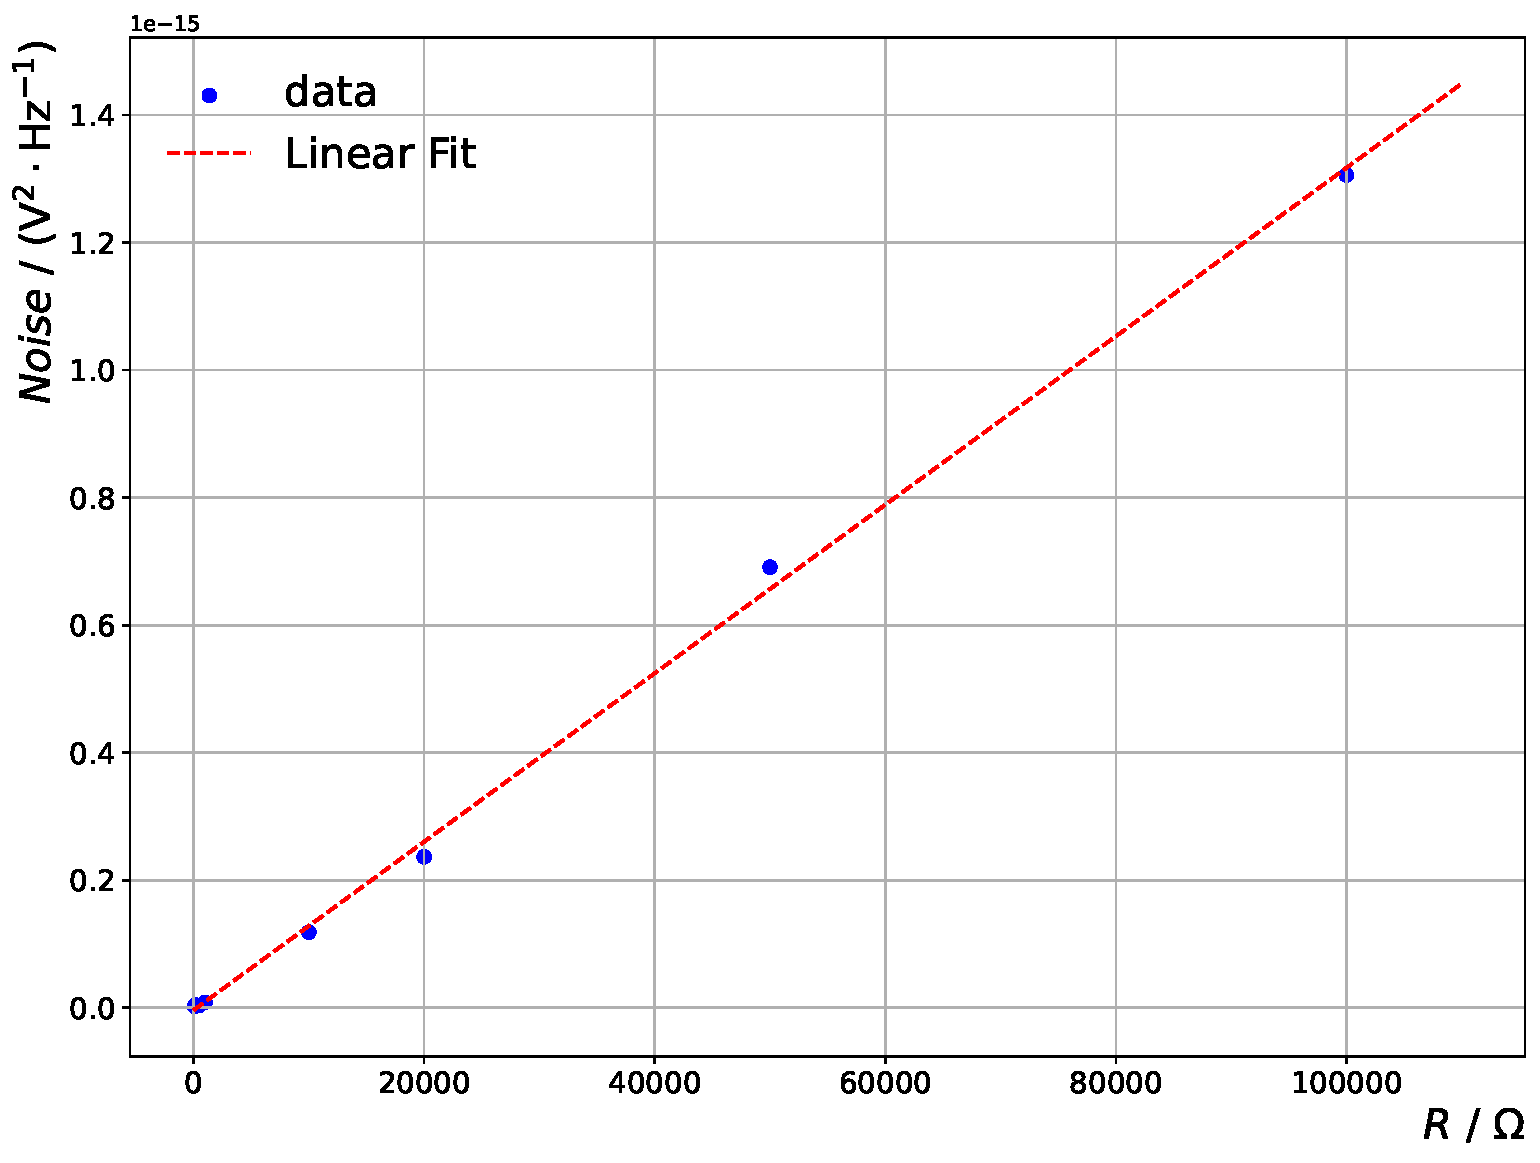
\includegraphics[height=12cm, width=16cm]{images/phyex1_fig1.pdf}
 \label{fig:fig3}
\end{figure}

通过线性拟合我们可以得到\textbf{图\ref{fig:fig3}}中直线斜率为
\begin{equation}
    4k_B T=1.3211\times 10^{-20}\si{V^2/\hertz}
\end{equation}

从而求得
\begin{equation}
    k_B=1.0973\times10^{-23}\si{J/K}
\end{equation}

小于标准值\(1.3806488(13)×10^{-23}\si{J/K}\)
\begin{comment}
如果需要索引参考文献,请使用\cite{Erdos01}, 同时已经将参考文献的项目模版在文末写出。
\end{comment}
%------------------------------------------------------------
\newpage
\subsection{散粒噪声的测量}\label{sub:2}
对于热噪声的测量,只需要把电阻盒两端的BNC接头接上一个“T”,然后分成两个通道接到差分放大器的输入.对于散粒噪声测量,需要一个简易的给小灯泡以及光电二极管供电的电路,放在屏蔽铝盒里面.

其中小灯泡是用一个1.5V的电池供电,通过一个可调电阻可以改变光照强度.光电二极管是通过一个9V的铅酸蓄电池供电,或者通过一个外接数字电源供电,但是用电源供电最好加一个隔地,避免引入额外的噪声.电池一般可以在噪声电路或者交流小信号电路看成是短路的.

根据理论我们有
\begin{equation}
    \frac{d\left<I^2\right>}{df}=2eI_{avg}
\end{equation}

即
\begin{equation}
    \frac{dU^2}{df}=2eRU
\end{equation}

经过数据处理,我们可以得到如下\textbf{图\ref{fig:fig4}}所示结果 
\begin{figure}[H]
 \centering
 \caption{散粒噪声大小随电压变化关系}
 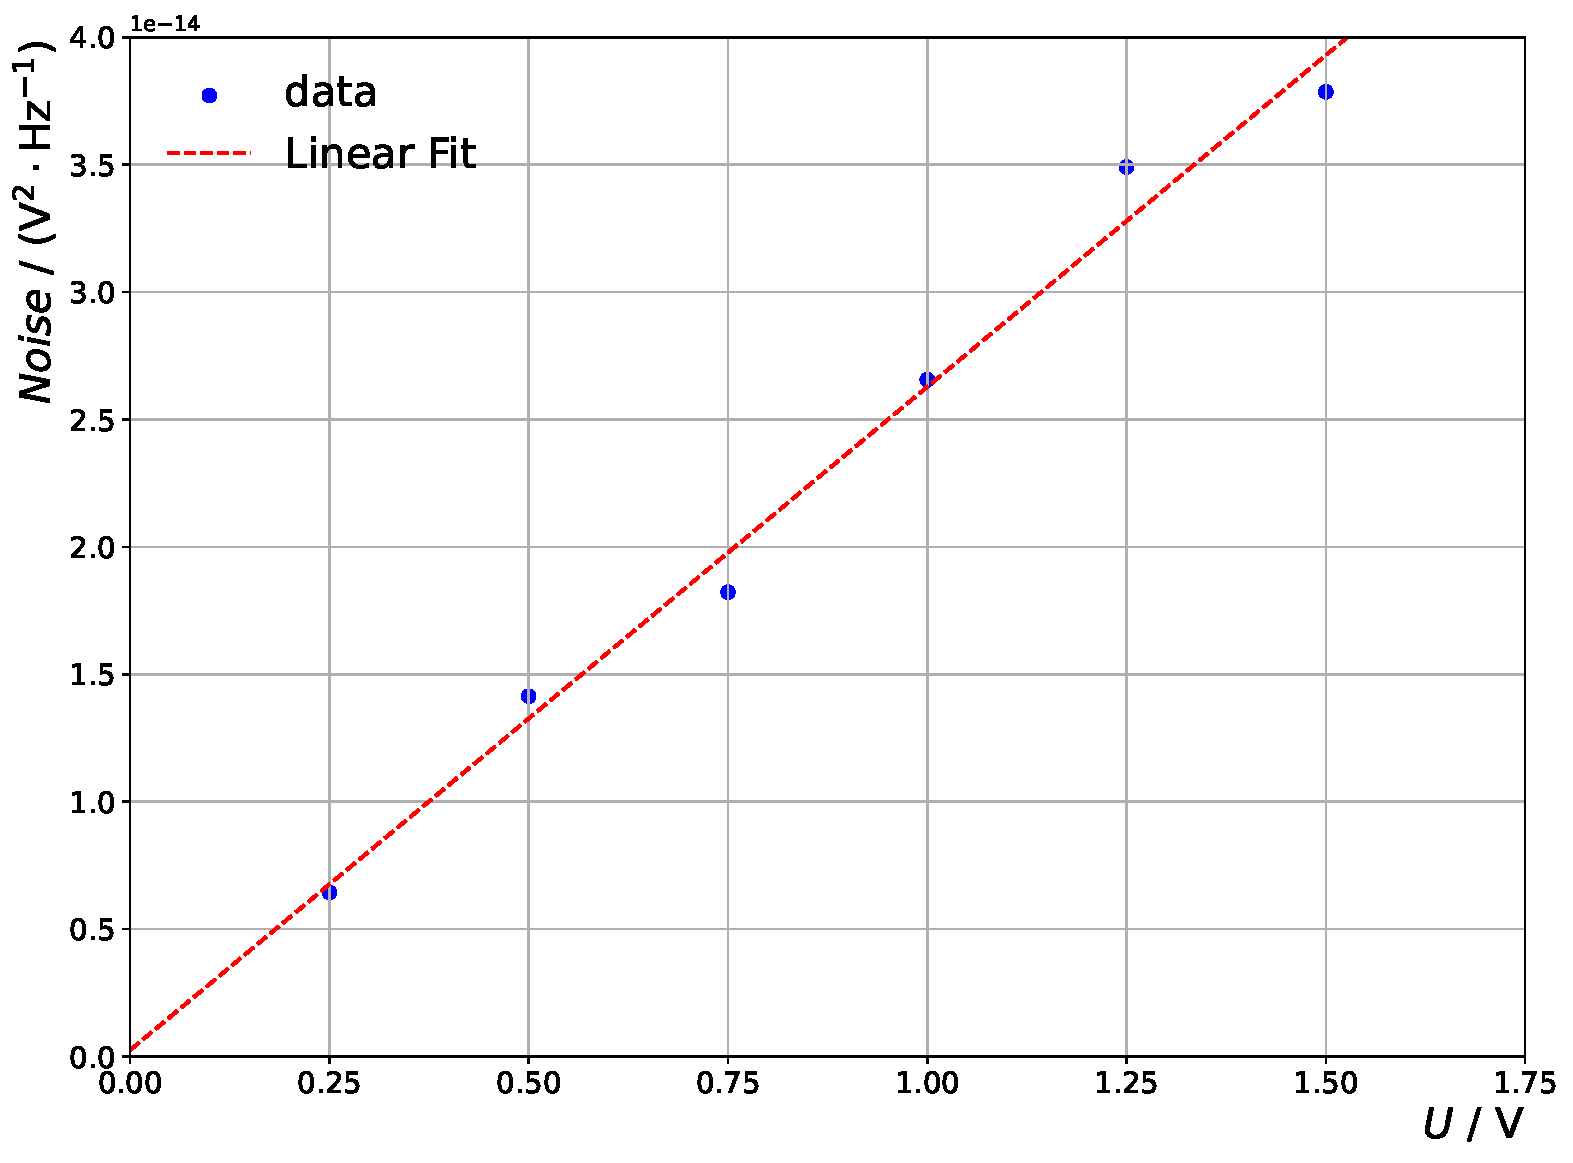
\includegraphics[height=12cm, width=16cm]{images/phyex1_fig2.pdf}
 \label{fig:fig4}
\end{figure}

通过线性拟合我们可以得到\textbf{图\ref{fig:fig3}}中直线斜率为
\begin{equation}
    2eR=2.6026\times 10^{-14}\si{V/\hertz}
\end{equation}

从而求得
\begin{equation}
    e=1.3013\times10^{-19}\si{C}
\end{equation}

小于标准值\(1.6022×10^{-19}\si{C}\)

%add more subsections for other block
%%%%%%%%%%%%%%%%%%%%%%%%%%%%%%%%%%%%%%%% Conclusion %%%%%%%%%%%%%%%%%%%%%%%%%%%%%%%%%%%%%%%%
\newpage
\section{结论}\label{conclusions}
本实验分为两部分,第一部分通过测量电阻上的热噪声来估算玻尔兹曼常数,第二部分通过测量光电二极管上的散粒噪声来估算电子的电荷,两个测量结果与标准值比起来都偏小,有待进一步的分析误差.

%%%%%%%%%%%%%%%%%%%%%%%%%%%%%%%%%%%%%%%% Questions %%%%%%%%%%%%%%%%%%%%%%%%%%%%%%%%%%%%%%%%
\begin{comment}
\section{实验报告思考题}\label{questions}
\subsection{在$a=23.0mm$、$b=10.0mm$的矩形波导管中能不能传播$\lambda=2cm$、$3cm$和$5cm$的微波?各能传播哪些波型?}\label{sub:question1}
答:根据
\begin{equation}
    \lambda_c=\frac{2}{\sqrt{(m/a)^2+(n/b)^2}}
\end{equation}
我们可以算出可传播的最大波长为$\lambda_{max}=18.3mm$,显然不能传播$\lambda=2cm$、$3cm$和$5cm$的微波,可传输波长在$\lambda_{max}=18.3mm$以下,满足$\lambda_c=\frac{2}{\sqrt{(m/a)^2+(n/b)^2}}$的波长的波型\\

\end{comment}

%%%%%%%%%%%%%%%%%%%%%%%%%%%%%%%%%%%%%%%% Acknowledgements %%%%%%%%%%%%%%%%%%%%%%%%%%%%%%%%%%%%%%%%

\section{致谢}\label{acknowledgments}
感谢老师在实验中的的悉心指导.

\begin{comment}
%%%%%%%%%%%%%%%%%%%%%%%%%%%%%%%%%%%%%%%% Appendix %%%%%%%%%%%%%%%%%%%%%%%%%%%%%%%%%%%%%%%%
\appendix
\section{代码}\label{sub:app.code}
请在附录\ref{sub:app.code}中添加代码。请使用如下Scala的语法高亮描述方法。
\begin{scala}
class TopIO extends Bundle() {
	val boot = Input(Bool()) 
// imem and dmem interface for Tests
	val test_im_wr		= Input(Bool())
	val test_im_rd 		= Input(Bool())
	val test_im_addr 	= Input(UInt(32.W))
	val test_im_in 		= Input(UInt(32.W))
	val test_im_out 	= Output(UInt(32.W))

	val test_dm_wr		= Input(Bool())
	val test_dm_rd 		= Input(Bool())
	val test_dm_addr 	= Input(UInt(32.W))
	val test_dm_in 		= Input(UInt(32.W))
	val test_dm_out 	= Output(UInt(32.W))

	val valid			= Output(Bool())
}
class Top extends Module() {
	val io 		= IO(new TopIO())//in chisel3, io must be wrapped in IO(...) 
	//...
	when (io.boot & io.test_im_wr){
		imm(io.test_im_addr) := io.test_im_in
		} .elsewhen (io.boot & io.test_dm_wr){
		// please finish it
		} //...
}
\end{scala}
\newpage

%%%%%%%%%%%%%%%%%%%%%%%%%%%%%%%%%%%%%%%% REFERENCE %%%%%%%%%%%%%%%%%%%%%%%%%%%%%%%%%%%%%%%%
\begin{thebibliography}{9}

\bibitem{Erdos01} P. Erd\H os, \emph{A selection of problems and
results in combinatorics}, Recent trends in combinatorics (Matrahaza,
1995), Cambridge Univ. Press, Cambridge, 2001, pp. 1--6.

\end{thebibliography}
\end{comment}
\end{document}

